\section{Perspective Projection}

\begin{figureBox}[label={fig:ortho-vs-persp}, width=0.8\linewidth]{Orthographic and perspective projections}
    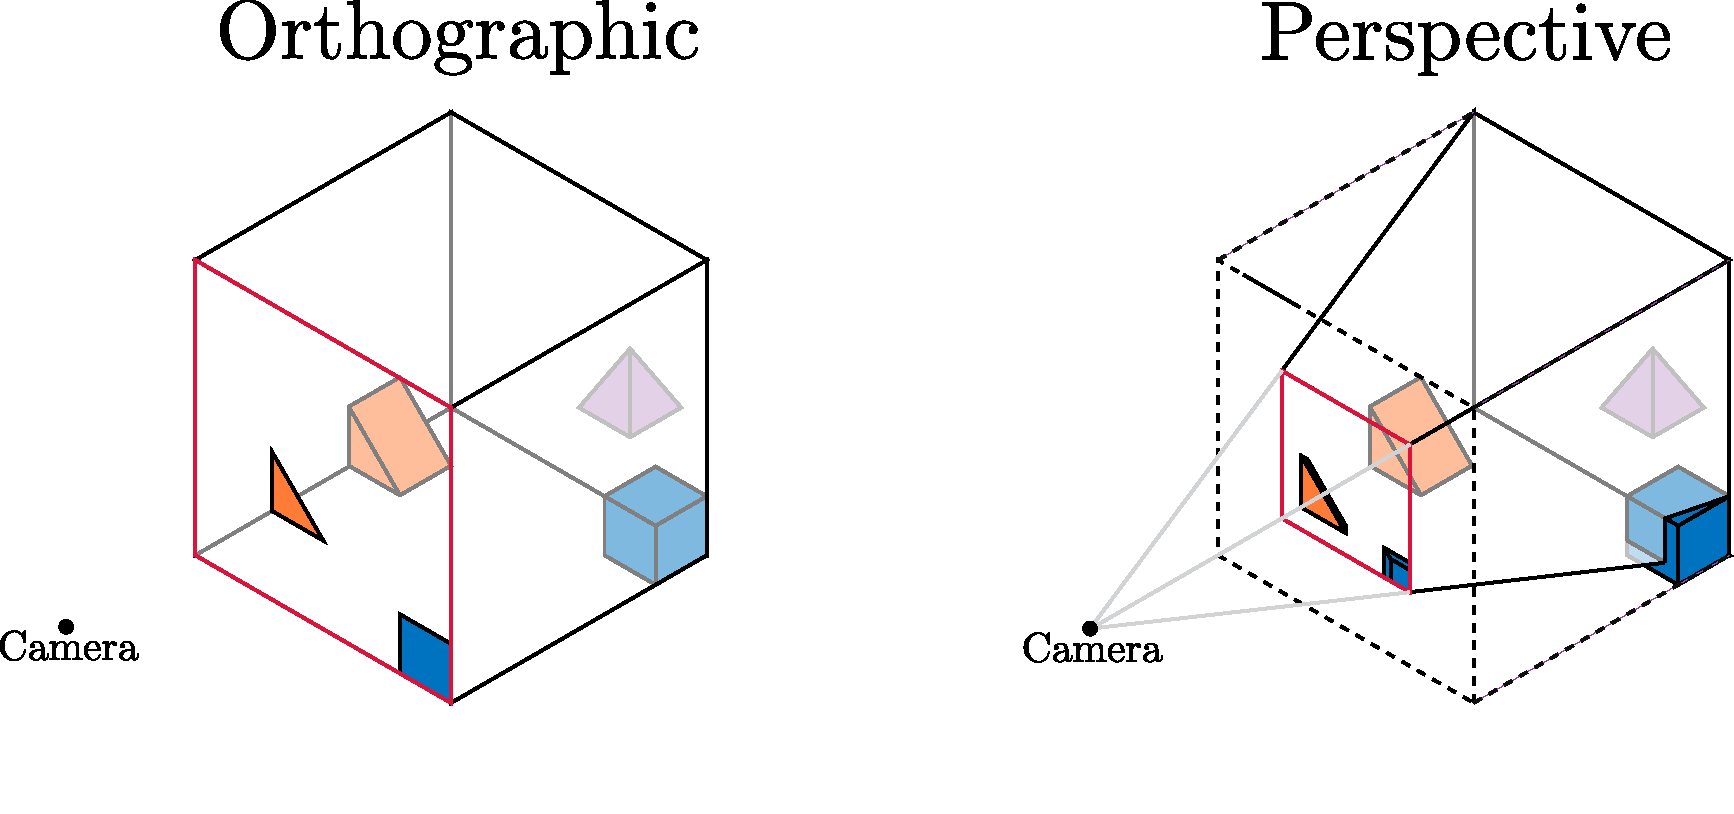
\includegraphics[width = 0.8\linewidth]{./background/figures/projection/ortho-vs-persp.pdf}
\end{figureBox}

To represent 3D objects on a 2D surface (our screen) OpenGL support two type of projections: perspective and orthographic as seen in Fig~\ref{fig:ortho-vs-persp}. Orthographic features parallel projection lines (orthogonal to the projection plane), which means that it does not depict the effect of perspective. Distances are preserved, making it useful for technical drawings where measurements need to be accurate and unskewed by perspective (All diagrams in this report are in the orthographic perspective). Unlike orthographic projection, perspective projection simulates the way the human eye perceives the world, with objects appearing smaller as they are farther from the viewpoint as the projection lines converge at a vanishing point. To create the illusion of 3D in this project we must use a perspective projection. \\

\begin{figureBox}[label={fig:persp-projection}, width=0.8\linewidth]{Using frustum to generate a perspective projection}
    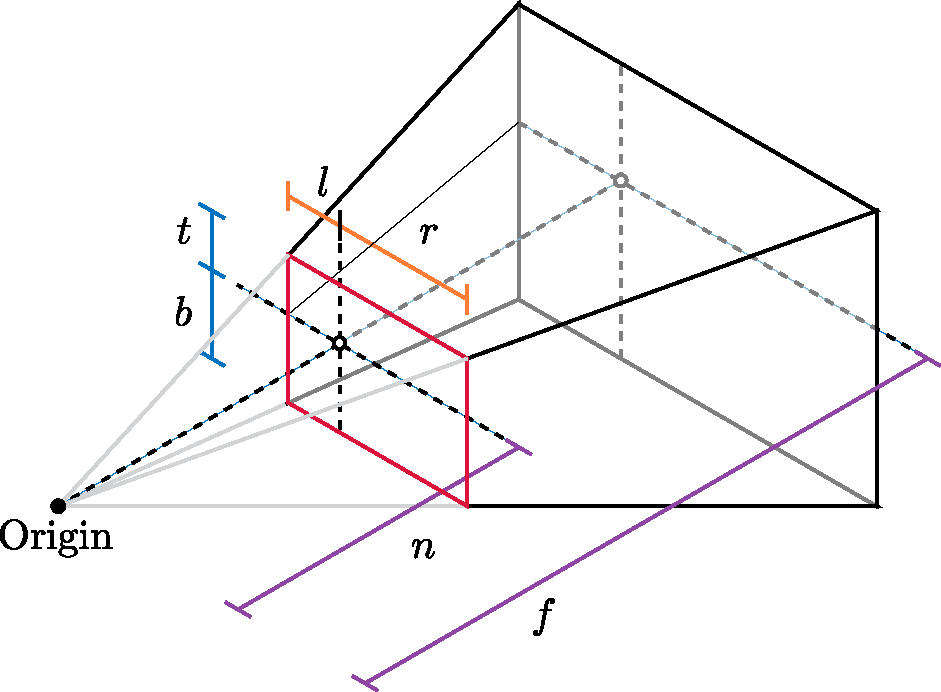
\includegraphics[width = 0.5\linewidth]{./background/figures/projection/persp-projection.pdf}
\end{figureBox}

OpenGL provides the \texttt{frustum} function as seen in Fig~\ref{fig:persp-projection} which can be used to construct a perspective matrix Fig~\ref{fig:perspective-matrix} that maps a specified viewing frustum  screen-space (with intermediate steps handelled by OpenGL) \tocite. The viewing frustum, is specified by six parameters: $f$, $l$, $r$, $b$, $t$, $n$ which represent left, right, bottom, top, near, and far. These parameters define the sides of the near clipping plane, highlighted in red, relative to the origin of the coordinate system. These parameters do not represent distances or magnitudes in a traditional sense but rather define the vectors from the center of the near clipping plane to its edges. \\

\begin{figure}[H]
    \[
        \begin{bmatrix}
            \frac{2n}{r-l} & 0              & \frac{r+l}{r-l}  & 0                \\
            0              & \frac{2n}{t-b} & \frac{t+b}{t-b}  & 0                \\
            0              & 0              & -\frac{f+n}{f-n} & -\frac{2fn}{f-n} \\
            0              & 0              & -1               & 0                \\
        \end{bmatrix}
    \]
    \caption{frustum perspective matrix}
    \label{fig:perspective-matrix}
\end{figure}

The $l$ and $r$ parameters specify the horizontal boundaries of the frustum on the near clipping plane, with left typically being a negative value and right a positive value, defining the extent to which the frustum extends to the left and right of the origin. Similarly, the $b$ and $t$ parameters determine the vertical boundaries, with bottom often negative and top positive, expressing the extent of the frustum below and above the origin. \\

The $n$ and $f$ parameters are scalar values that specify the distances from the origin to the near and far clipping planes along the view direction. Altering the value of $n$ will change the angles of the lines (or vectors) that connect the corners of the near plane to the eye, effectively changing the "field of view". Changing the value $f$ affects the range of depth that is captured within the scene. \\

If we are able to track the position of a viewers eye in real time then we can create the illusion of a 3D scene behind and in front of a display using \texttt{frustum}. This can be done fairly trivially following Robert Kooima's method he sets out in "Generalised Perspective Projection" to calculate $f$, $l$, $r$, $b$, $t$, $n$ as the viewers eye moves \cite{kooima2009generalized}. \\



To encode the position and size of the screen we take 3 points, $p_a$, $p_b$ and $p_c$ which represent the lower-left, lower-right and upper left points of the screen respectively when viewed from the front on. These points are in tracker space, the co-ordinate system of the device we use to track the eyes. These point can be used to generate an orthonormal basis of the screen of $s_r$, $s_u$ and $s_n$ which represents the directions up, right and normal to the screen respectively as seen in Fig~\ref{fig:perspective-screen}. We can compute these values from the screen corners as follows:
\[s_r = \frac{p_b-p_a}{||p_b-p_a||} \quad s_u = \frac{p_c-p_a}{||p_c-p_a||} \quad s_n = \frac{s_r\times s_u}{||s_r \times s_u||}\]

\begin{figureBox}[label={fig:perspective-screen}, width=0.8\linewidth]{Defining a screen in 3D space}
    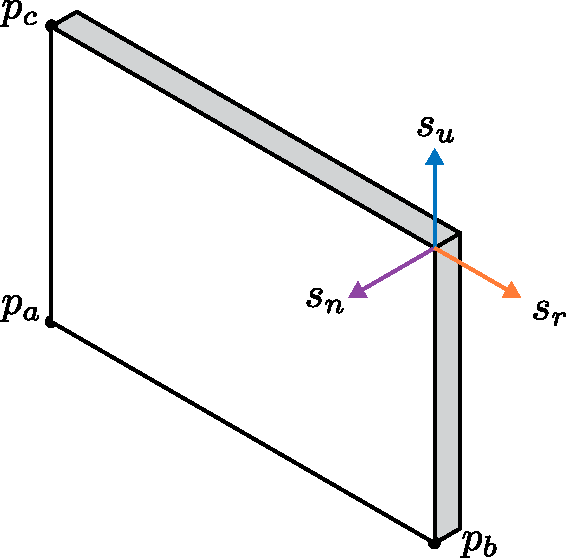
\includegraphics[width = 0.3\linewidth]{./background/figures/projection/screen.pdf}
\end{figureBox}

Introducing the viewers eye which we will refer to as $p_e$. We can draw three vectors $v_a$, $v_b$, $v_c$ from the viewers eye $p_e$ to the corners of the screen $p_a$, $p_b$, $p_c$ as seen in Fig~\ref{fig:screen-extents}. In the diagram we also have labelled the components of each of these vectors in the basis of the screen. We can compute these as follows:
\[ v_a = p_a - p_e \quad v_b = p_b - p_e \quad v_c = p_c - p_e\] \\

To calculate the required values for \texttt{frustum} we must first find the point where line drawn perpendicular to the plane of the screen that passes through $p_e$ strikes the plane of the screen. We refer to this point as the {\it screen-space-origin}, it is worth noting that this point can lie outside the screen (the rectangle bounded by $p_a$, $p_b$, $p_c$). We can find the distance of the {\it screen-space-origin} from the eye $p_e$ by taking its component of any of $v_a$, $v_b$, $v_c$ in the screen basis vector $s_n$, however as $s_n$ is in the opposite direction we must invert it. Similarly we can calculate $t$ by taking the component of $v_c$ in the basis vector $s_u$, $b$ by $v_b$ in $s_u$, $l$ by $v_c$ in $s_r$ and lastly $r$ by $v_b$ in $s_r$. We can compute these as follows:
\[ d= -(s_n \cdot v_a) \quad l = (v_c \cdot s_r) \quad r = (v_b \cdot s_r) \quad b = (v_c \cdot s_u) \quad t = (v_b \cdot s_u) \]

\begin{figureBox}[label={fig:screen-extents}, width=0.8\linewidth]{Screen Intersection with view}
    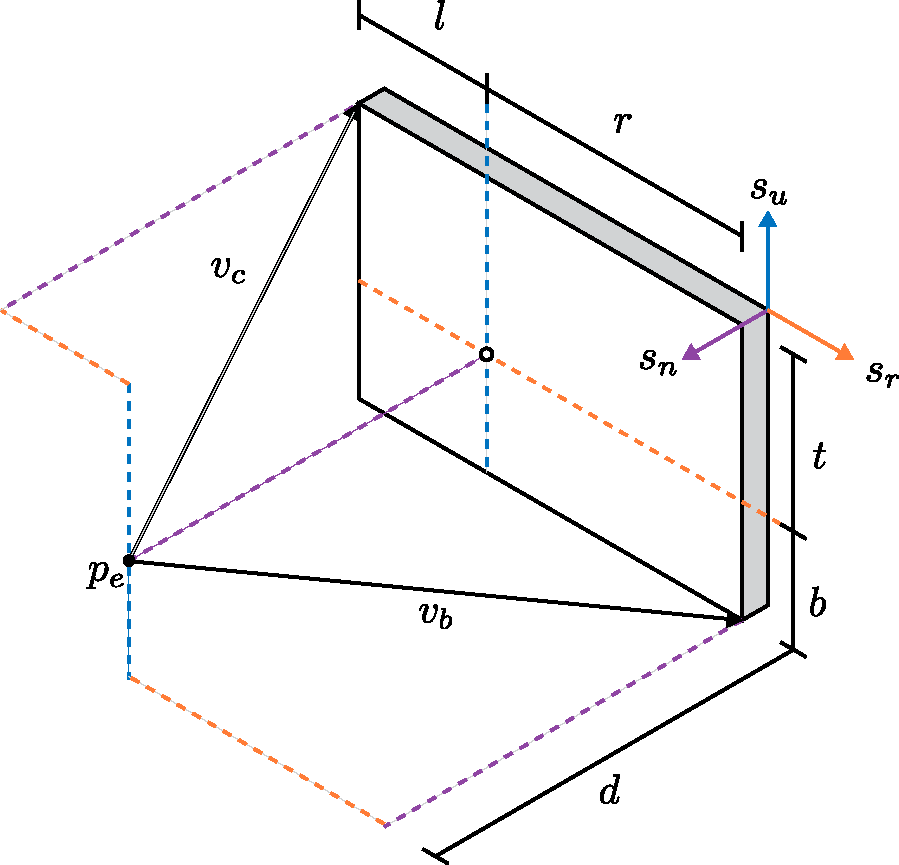
\includegraphics[width = 0.5\linewidth]{./background/figures/projection/eye-projection.pdf}
\end{figureBox}

We can now generate a projection matrix by calling \texttt{frustum} using $d$ as our nearClipping plane distance $n$ with an arbitrary value for the farClipping plane $f$. We have now successfully generated our viewing frustum but we still have two problems. Firstly our frustum has been defined in tracker space so is pointed in the direction of our camera not the normal of our screen. We can remerdy this problem by using a rotation matrix M to align our frustum with $s_n$, $s_u$ and $s_r$, the basis of our screen as seen in Fig~\ref{fig:basis-change}. M is defined as follows:
\[
    \begin{bmatrix}
        v_{rx} & v_{ry} & v_{rz} & 0 \\
        v_{ux} & v_{uy} & v_{uz} & 0 \\
        v_{nx} & v_{ny} & v_{nz} & 0 \\
        0      & 0      & 0      & 1 \\
    \end{bmatrix}
\]

\begin{figureBox}[label={fig:basis-change}, width=0.8\linewidth]{Moving the frustum from tracker space to screen space}
    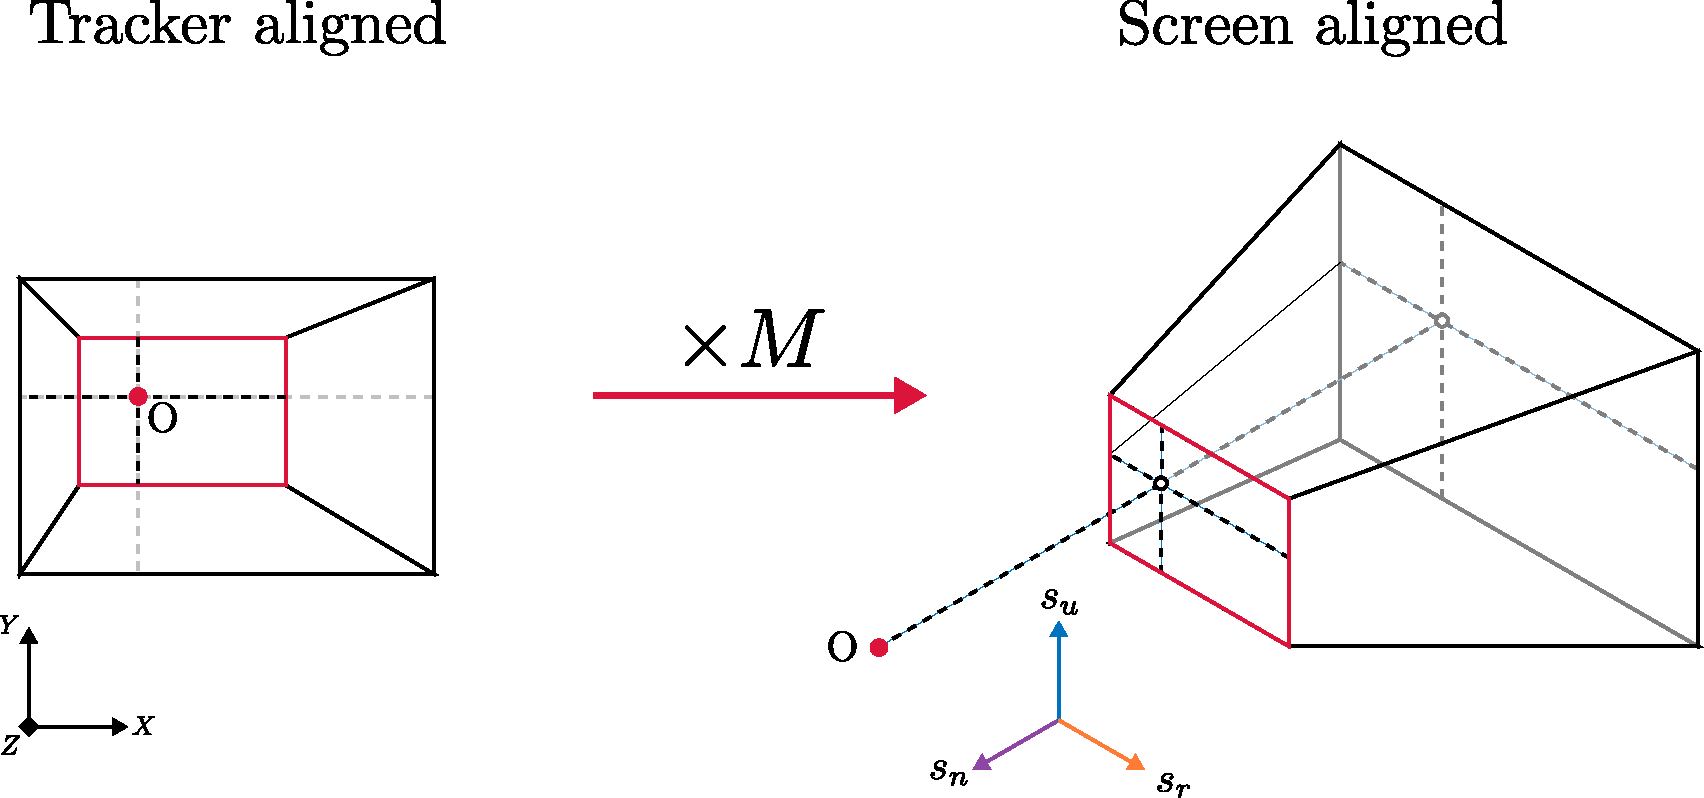
\includegraphics[width = 0.8\linewidth]{./background/figures/projection/realignment.pdf}
\end{figureBox}

The second problem we have is that we want our projection matrix to move around with the viewers eye however the mathematics of perspective projection disallow this, with the camera forever trapped at the origin. To translate our viewing frustum to our eye position we must instead translate our eye position (and the whole world) to the apex/origin of our frustum. This can be done with a translation matrix $T$ as seen in Fig~\ref{fig:frust-translation}. $T$ $T$ can be generated with the OpenGL function \texttt{translate} where we want to offset it by the vector from our Origin to the viewers eye $p_e$. T is defined as follows:
\[
    \begin{bmatrix}
        1 & 0 & 0 & -p_{ex} \\
        0 & 1 & 0 & -p_{ey} \\
        0 & 0 & 1 & -p_{ez} \\
        0 & 0 & 0 & 1       \\
    \end{bmatrix}
\]

\begin{figureBox}[label={fig:frust-translation}, width=0.8\linewidth]{Translating the viewing frustum to sit inside the screen}
    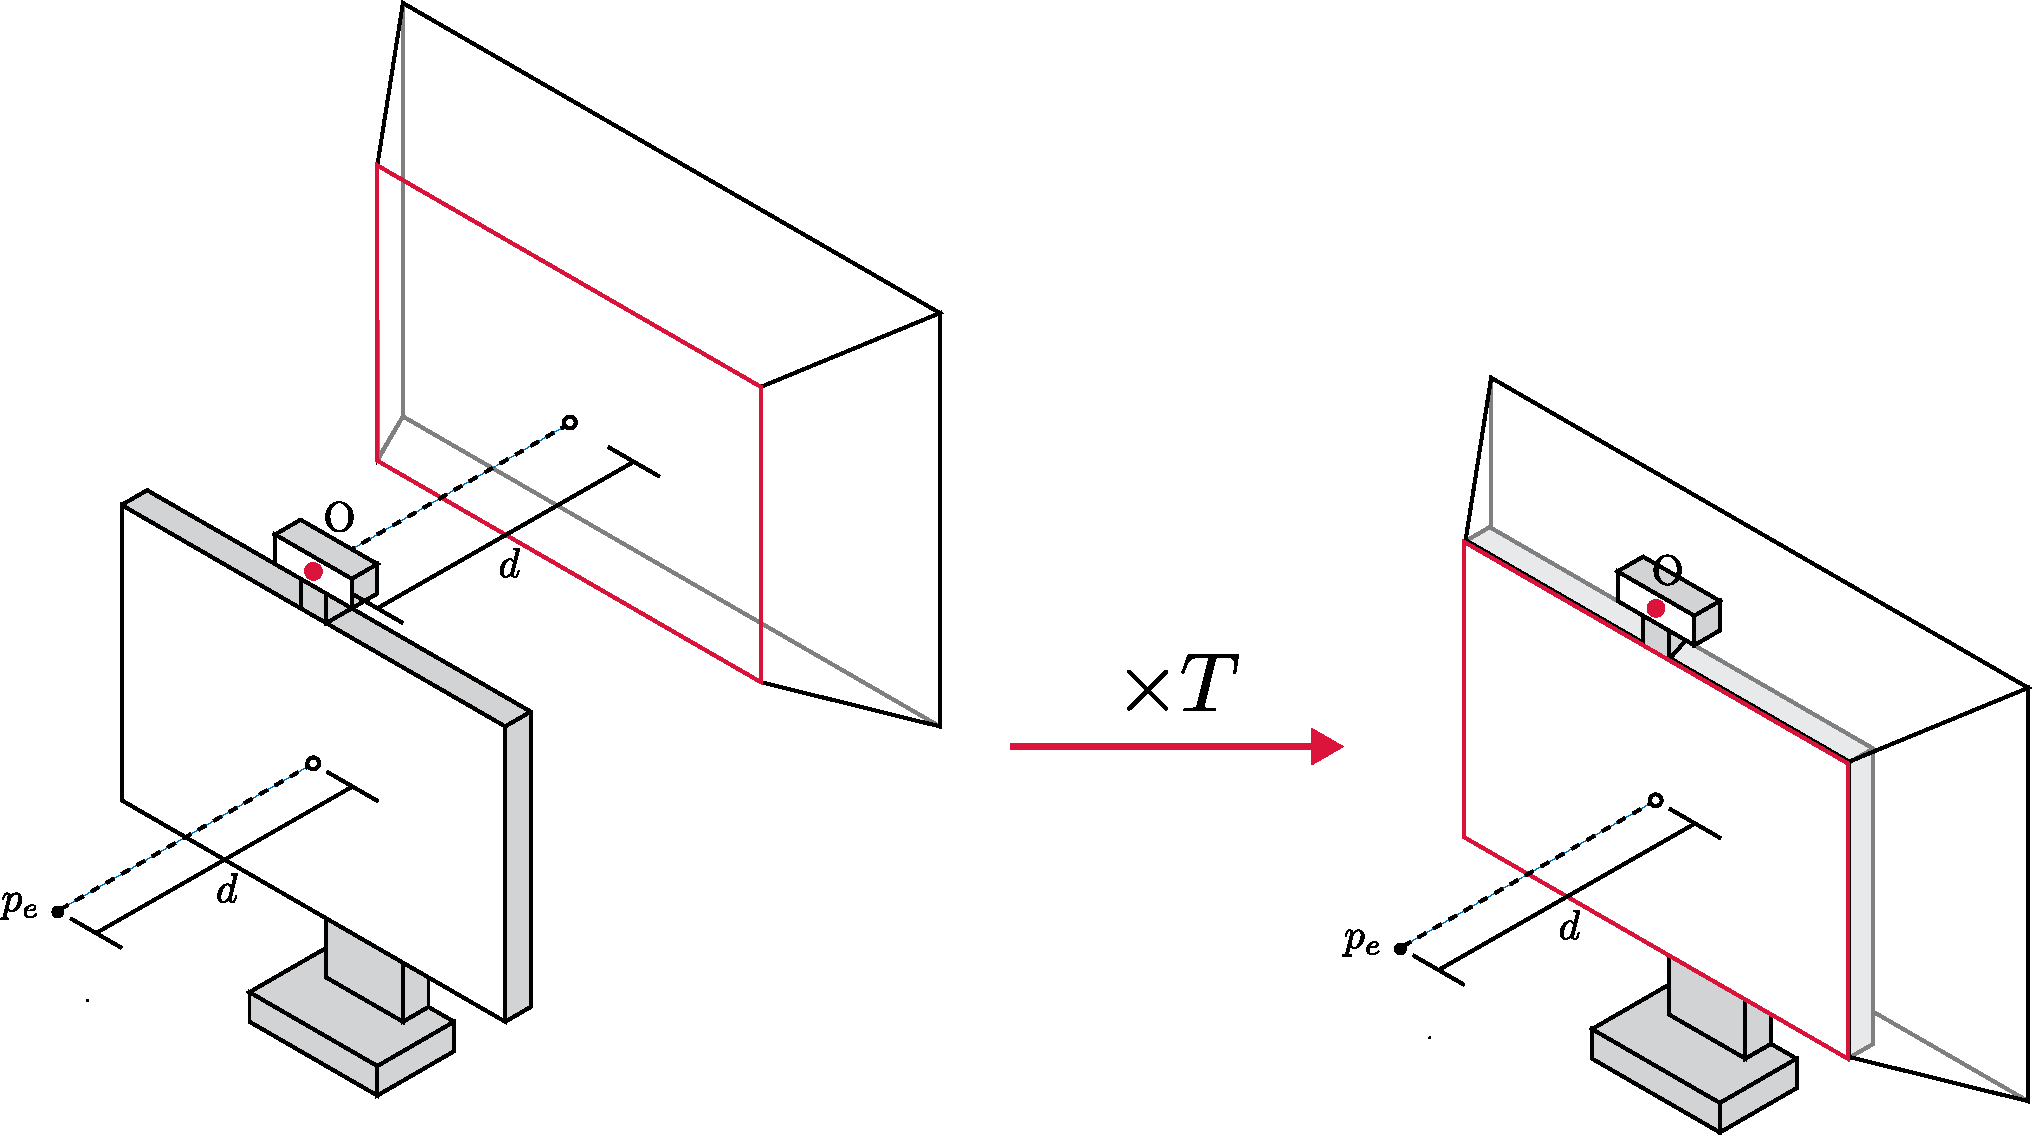
\includegraphics[width = 0.8\linewidth]{./background/figures/projection/frust-translation.pdf}
\end{figureBox}

We now have a working method for projecting virtual objects behind our screen onto our screen however it is also possible if we desire to project objects in front of the screen onto the screen as well as long as they lie within the pyramid formed between the edges of the screen and the viewers eye. We can use similar triangles to scale near clipping plane from the plane of the screen to a small distance $n$ from our eye as seen in Fig~\ref{fig:extending-near}. We now have scaled down values of $t$, $b$ $l$ and $r$ we can use for our new viewing frustum which we call $t_n$, $b_n$ $l_n$ and $r_n$. They are defined as follows:
\[
    l_n = (v_c \cdot s_r) \frac{n}{d} \quad r_n = (v_b \cdot s_r) \frac{n}{d} \quad b_n = (v_c \cdot s_u) \frac{n}{d} \quad t_n = (v_b \cdot s_u) \frac{n}{d}
\]

So our final viewing frustum takes in frustum extents $t_n$, $b_n$ $l_n$ and $r_n$ and $n$ and $f$ defining the distances to the near and far clipping plane.
\begin{figureBox}[label={fig:extending-near}, width=0.8\linewidth]{Extending the near plane to not clip out objects in front of the screen}
    \centering
    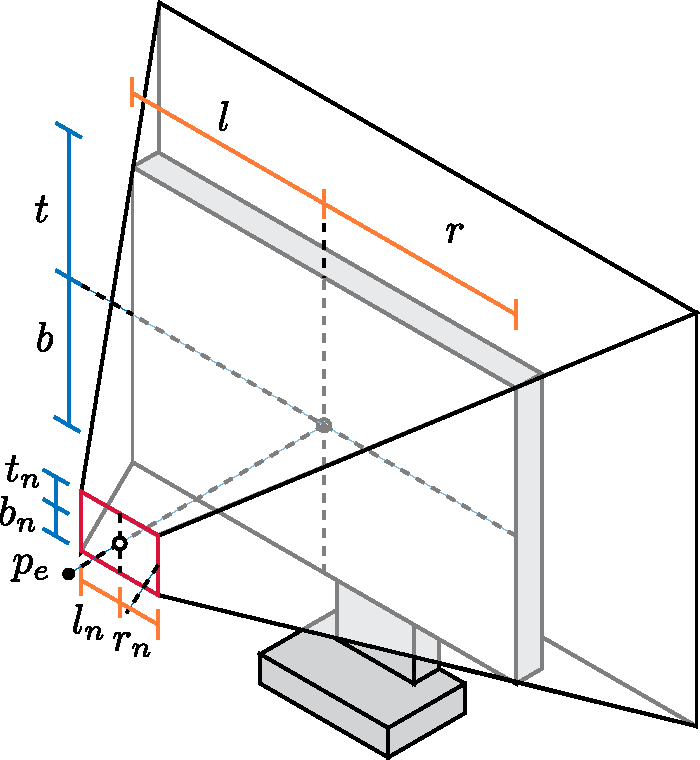
\includegraphics[width = 0.5\linewidth]{./background/figures/projection/extending-near.pdf}
\end{figureBox}


Below we have attached some sample code of a function implementing the process we just described.

\codeBoxFile{cpp}{./background/code/projection.cpp}{projection.cpp, Sample code for creating the 3D illusion projection}
